\documentclass[a4paper,12pt]{article}
\usepackage{graphicx}
\usepackage{hyperref}
\begin{document}

\centerline{\huge \textbf{Implementation documentation}} \hspace*{\fill}

This document studies the \emph{data structures} and \emph{algorithms} used in the program, reports their \emph{time} and \emph{memory requirements} as for their current \emph{implementations}. \emph{Flaws} of the implementation are also mentioned.
\paragraph{\large Queue} \hspace{0pt} \\
\\
Implemented methods: \emph{enqueue, dequeue, peek, clear, isEmpty, size, toLinkedList}\\
\\
All methods for this data structure only perform \emph{simple value assignments}, some of them with \emph{if-checks}. That way all Queue's actions are done in \emph{constant time} and with \emph{constant memory}. \emph{enqueue} creates a new object, which still requires constant memory. \emph{toLinkedList} method is an exception, as its time and memory requirement is O(n), where \emph{n} is amount of \emph{elements} in the Queue. Besides the elements, Queue only needs to store a constant amount of variables. So, overall, memory requirement for the Queue is O(n).
\\

\paragraph{\large LinkedList} \hspace{0pt} \\
\\
Implemented methods: \emph{add, clear, isEmpty, reset, hasNext, getNext, size}\\
\\
All methods for this data structure only perform simple value assignments, some of them with if-checks. That way all LinkedList's actions are done in constant time and with constant memory. \emph{add} creates a new object, which still requires constant memory. Besides the elements, LinkedList only needs to store a constant amount of variables. So, overall, memory requirement for the LinkedList is O(n) where \emph{n} is amount of elements in the LinkedList.\\
\emph{remove} method was not implemented, as the use of LinkedList in this project didn't need to remove specific elements on the LinkedList. Because the method would require O(n) time to find the element and its predecessor as elements are \emph{linked} in one way, it would be better to use a Tree if removing elements is required.
\\

\paragraph{\large Tree} \hspace{0pt} \\
\\
Implemented methods: \emph{add, remove, getMin, clear, isEmpty, contains, size, toLinkedList}\\
\\
Implemented Tree is \emph{self-balancing} using the \emph{red-black principle}. Implementation mimics the guidelines presented in the Wikipedia article: \url{http://en.wikipedia.org/wiki/Red-black_tree} Custom \emph{comparator} class can be used to compare elements in a desired way.\\

\textbf{add:} First, tree finds a suitable \emph{placement} for the new element. In worst case scenario, the placement in question may be found at the bottom of the tree. Because tree's height is below 2 * log(n) (\emph{n} = amount of elements), finding the placement requires O(log(n)) time. After that several tree \emph{balancing techniques} are used depending on a specific \emph{scenario}. Most techniques require constant time, however one scenario requires to iterate the balancing techniques for added \emph{node's parent}. Balancing on addition requires O(log(n)) time. Overall, time requirement is O(log(n)). Memory requirement is constant.
\\

\textbf{remove:} Deleted element first must be \emph{found}, which requires O(log(n)) time. Some balancing techniques are performed in constant time, others \emph{iterate upwards}, requiring O(log(n)) time.  Overall, time requirement is O(log(n)). Memory requirement is constant.
\\

\textbf{contains:} Required element may be a \emph{leaf} of the Tree, in which case finding it requires O(log(n)) time. Same time is required, if Tree doesn't contain given element. Overall, time requirement is O(log(n)). Memory requirement is constant.
\\

\textbf{toLinkedList:} All elements are traversed \emph{breadth first} using the Queue. Each element is processed once, so required time is O(n). Elements need to be stored in Queue and the LinkedList, which the method will return. Overall memory requirement is O(n)
\\

\emph{getMin, clear, isEmpty} and \emph{size} perform at constant time and memory. Besides the elements, Tree only needs to store a constant amount of variables, making overall memory requirement O(n).\\
\\
Tree can be extended to act as a \emph{map} that holds \emph{key-value pairs}. Overall memory requirement is not changed in \emph{O-notation}.\\

\textbf{get:} finds the \emph{key} element and returns its \emph{value}. Time requirement O(log(n)), memory requirement constant.
\\

\textbf{put:} Calls \emph{contains} method. If element is contained, elements value is changed. If not, \emph{add} is called to add a new element to the tree. Time requirement O(log(n)), memory requirement constant.
\\

There is a flaw in the implementation. Suppose we have elements \emph{a} and \emph{b}. If Tree's comparator's values for both comparisons are on the same side from zero (compare(a,b) * compare(b,a) $\geq{0}$), these elements cannot be \emph{differentiated}. This may lead to many unexpected results. If comparator classes have to be customly implemented, compare method shouldn't return zero, unless programmer is willing to assume that if compare(a,b) = 0, then \emph{a} and \emph{b} are considered to be the \emph{same} element.

\paragraph{\large Graph} \hspace{0pt} \\
\\
While Graph is not explicitly coded in the program, Graph is implemented with Vertex objects and VertexContainer, which contains all created vertices. Vertex keeps its adjacent vertices in a Tree, and VertexContainer keeps vertices in a Tree. VertexContainer stores \emph{v} amount of memory and sum of all stored adjacent vertices for every vertex is \emph{e}, where \emph{v} is amount of vertices and \emph{e} is amount of edges. Overall memory requirement O(v+e).
\\

\paragraph{\large Heap} \hspace{0pt} \\
\\
Implemented methods: \emph{insert, pop, peek, clear, isEmpty, size, valueChanged}.
\\
Heap in question is a \emph{binary tree}, which stores elements in an \emph{array}. Custom comparator class can be used to compare elements in a desired way. Heap can be paired with a TreeMap, which returns given element's \emph{index value} in heap's array.\\

\textbf{insert:} Added element's \emph{location} in the Heap is found, which takes O(log(n)) time. Element is placed to the end of the array, after which it is \emph{swapped} with the \emph{parent} if Heap rules are violated. On each swap, TreeMap's value is changed, which also takes O(log(n)) time. When placement is found, TreeMap's value is changed one more time. Overall, time requirement with a TreeMap is O($log^{2}$(n)), without it it's O(log(n)). Memory requirement is O(1). However, because Heap stores its data in a \emph{finite} array, if array is \emph{overflown}, elements must be copied into a bigger array (this implementation doubles the size of the array). Increasing array takes O(n) time and memory. However, the array is increased at exceptional situations. So, overall, time requirement is O($log^{2}$(n)) and memory requirement is O(1).
\\

\textbf{pop:} First element in the Heap is replaced by the last element, which is then swapped with one of the childs if heap rules are violated. This takes O(log(n)) time without TreeMap, with it it's O($log^{2}$(n)) as TreeMap is updated on every swap. Memory requirement is O(1).
\\

\textbf{valueChanged:} First, element's index is searched from the treeMap, which takes O(log(n)) time. Then, element is moved up or down on the heap at a correct position in the heap. On eaxh position swap, TreeMap is updated. Overall, time requirement is O($log^{2}$(n)) and memory requirement is O(1).
\\

\emph{peek, clear, isEmpty} and \emph{size} perform at constant time and memory. Heap allocates memory for elements in the array and TreeMap. Heap also has constant amount of variables. Overall, memory requirement for the Heap is O(n).\\
Heap has same flaws with comparators as with the Tree. When pairing Heap with TreeMap, each data structure should use a different \emph{comparator class}. The values that Heap's comparator \emph{compares} can be assumed to change, while TreeMap's compared values must stay \emph{fixed} throughout the use of the Heap. 

\paragraph{\large Path finding with Dikstra's algorithm} \hspace{0pt} \\
\\
Algorithm's rough progression:\\
\\
1. Algorithm places all vertices in a Heap and a TreeMap of \emph{distance estimates}, where every estimate is MAXVALUE except for the \emph{starting vertex}, whose estimate is 0. Heap's comparator accesses the TreeMap with distance estimates, that way vertex with smallest distance estimation is \emph{on top}.\\
2. Vertex is \emph{popped} from the Heap, all of its \emph{adjacent} vertices are iterated, and their distances are re-estimated. Because comparator's \emph{compare} method uses Treemap's \emph{get} method, this increases Heap's \emph{poll} method's time requirement to O($log^{3}$(n)). Now every adjacent vertex stores popped vertex as its previous point in the path.\\
3. Repeat 2 until Heap is empty. Now we have found all shortest paths from a given starting vertex. Overall time requirement is O((v + e) * $log^{3}$(v)), where \emph{v} is amount of vertices and \emph{e} is amount of edges in the graph. Memory requirement is O(v).\\
\\
Implemented algorithm mimics A* by using a simple \emph{heuristic} to check less edges in the graph. Heuristic in question is \emph{chebyshev distance}. Vertices with smaller chebyshev distance are preferred to vertices with bigger chebyshev distance. Algorithm \emph{terminates} itself when end vertex is popped from the heap.\\
Implemented algorithm requires more than O((v + e) * log(v)) time, which is widely considered to be Dijkstra's algorithm's requirement. To achieve that time, TreeMap should be replaced with HashMap for Heap's index retrieval and keeping distance estimations. Hashmap's \emph{get} and \emph{put} methods perform at constant time instead of logarithmic time.

\paragraph{\large Graph building with tracing} \hspace{0pt} \\
\\
Tracing algorithm was largely underestimated in the requirements documentation. Algorithm's rough progression: \\
\\
1. Choose a vertex \emph{v} from which point of view other vertices are traced.\\
2. Choose another point \emph{p}. Store the \emph{direction} and \emph{distance} from \emph{v} to \emph{p}. Also store direction and distance from \emph{v} to \emph{p.right}, assuming that \emph{p} is a part of a \emph{polygon} and thus has a connection with a \emph{left and right neighbour}, all of which are a part of the same polygon. This data can be represented as a \emph{sector} of two directions.\\
3. Repeat 2 for every \emph{point} in the field. Sectors are stored in a Heap, where a sector with the smallest \emph{left direction value} is placed on top of the Heap. Time requirement: O(p * log(p)) Memory requirement: O(p), where \emph{p} is amount of geometry points.\\
4. Go through the sectors and remove \emph{redundant and overlapping} sectors. Each stored sector is pulled from the Heap (Time: O(p * log(p))) and stored in a Tree (Time: O(p * log(p))), where sectors closest to the \emph{v} are stored as a \emph{left child}. Using this technique, amount of stored sectors is reduced significantly, where sector amount is \emph{s} and s $\leq{p}$. Memory requirement: O(p).\\
5. All vertices are checked whether they are \emph{obstructed} by any sector. Time requirement: O(r * s), where \emph{r} is amount of points with \emph{reflex angles} (which is less than or equals \emph{p}) and \emph{s} is amount of usable sectors (also less than \emph{p}). Memory requirement: O(q), where \emph{q} is amount of points that are unobstructed to the \emph{v}. That way q $\leq{p}$.\\
6. Repeat this for every \emph{v} in the field.\\
\\
Overall time requirement: O(v * ((p * log(p)) + (r * s))), where \emph{v} is amount of all vertices in the field, regardless if they are part of some polygon. That way p $\leq{v}$, also we have established that r $\leq{p}$ and s $\leq{p}$. So, in worst case scenario, we could argue that the time to rebuild the graph is:\\
O(v * (p * log(p) + $p^{2}$)) = O($v^{2}$ * log(v) + $v^{3}$) = O($v^{3}$).\\
In current implementation, it is fair to assume that \emph{v = p}, because with currently implemented tools user can only place two vertices, which are not a part of any polygon. To assume that \emph{r = p} is a bit of a stretch, however that will happen if user decides to have all of the polygons to be \emph{reflex}. The interesting bit is studying the relation between \emph{s} and \emph{p}.\\
Because s $\leq{p}$, we can represent the relation as: \emph{s = c * p}, where \emph{c} $\geq{0}$ and c $\leq{1}$. This histagram shows the value of \emph{c} retrieved by \emph{empirical} means.\\ \\
\centerline{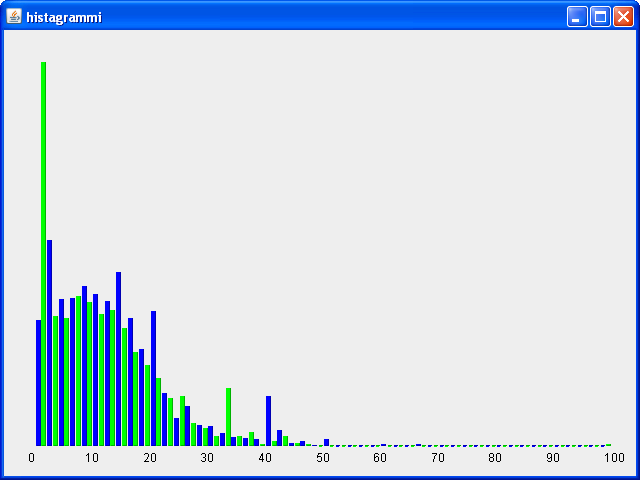
\includegraphics[scale=0.5]{histagram.png}} \hspace*{\fill} \\
This data was collected from 55672 occurences. X-axis represents the value of \emph{c} (in percents), and height of a column shows how many occurences fit the particular \emph{value interval}. We can see that \emph{c} hardly reaches above 0.5 and has a distinct peak at [0.1, 0.2]. This suggests that equating \emph{s} with \emph{p} isn't entirely fair. Now time requirement looks like: O($p^{2}$ * (log(p) + c))\\
Memory requirement: O(p). At any stage of the algorithm no more than p amount of memory allocation is required.\\
Built graph is redundant in many places, hurting the performance. However, the means to detect these redundancies may hurt the performance as badly. Perhaps a different approach to tracing would take less time in expense of more memory requirement. If field was divided into a \emph{grid}, where each rectangle stores all lines that \emph{intersect} it (allowing the same line to be stored in several rectangles), each trace would check appropriate areas of the field for intersections with other lines. Line candidates would be reduced, taking less time for tracing, however memory load would increase.

\end{document}